\subsection{DC Sweep desde $-V_{CC}$ hasta $V_{CC}$}
%Buscar valor maximo en hoja de datos vcc aprox 17 creo.BUSCAR voutMAX!!!
Dado que se nos pidi\'o alimentar al amplificador operacional con $V_{CC} = \pm 15V$, un DC Sweep desde $-V_{CC}$ hasta $V_{CC}$ requerir\'ia $30V_{pp}$ del generador de se\~nales. Una limitaci\'on de los generadores del laboratorio es que alcanzan un m\'aximo de $20V_{pp}$, por lo que no podr\'iamos llevar a cabo las mediciones generando una rampa en el rango de tesniones mencionado. La desici\'on tomada para lograr lo pedido fue, en el dise\~no del circuito, agregarle una etapa previa de amplificaci\'on utilizando otro amplificador operacional. 
El amplificador operacional no permite amplificar mas de un valor determinado, y por lo tanto no hay forma de llegar exactamente a -15V y a 15V a la entrada del circuito ya que su tensi\'on de entrada es la salida del amplificador operacional empleado en la etapa previa de amplificaci\'on de la se\~nal del generador.

\subsubsection*{Configuraci\'on inversora} %%%%%%%%%%%%%%%%%%%%%%%%%%

\begin{figure}[H] %!ht
	\centering
	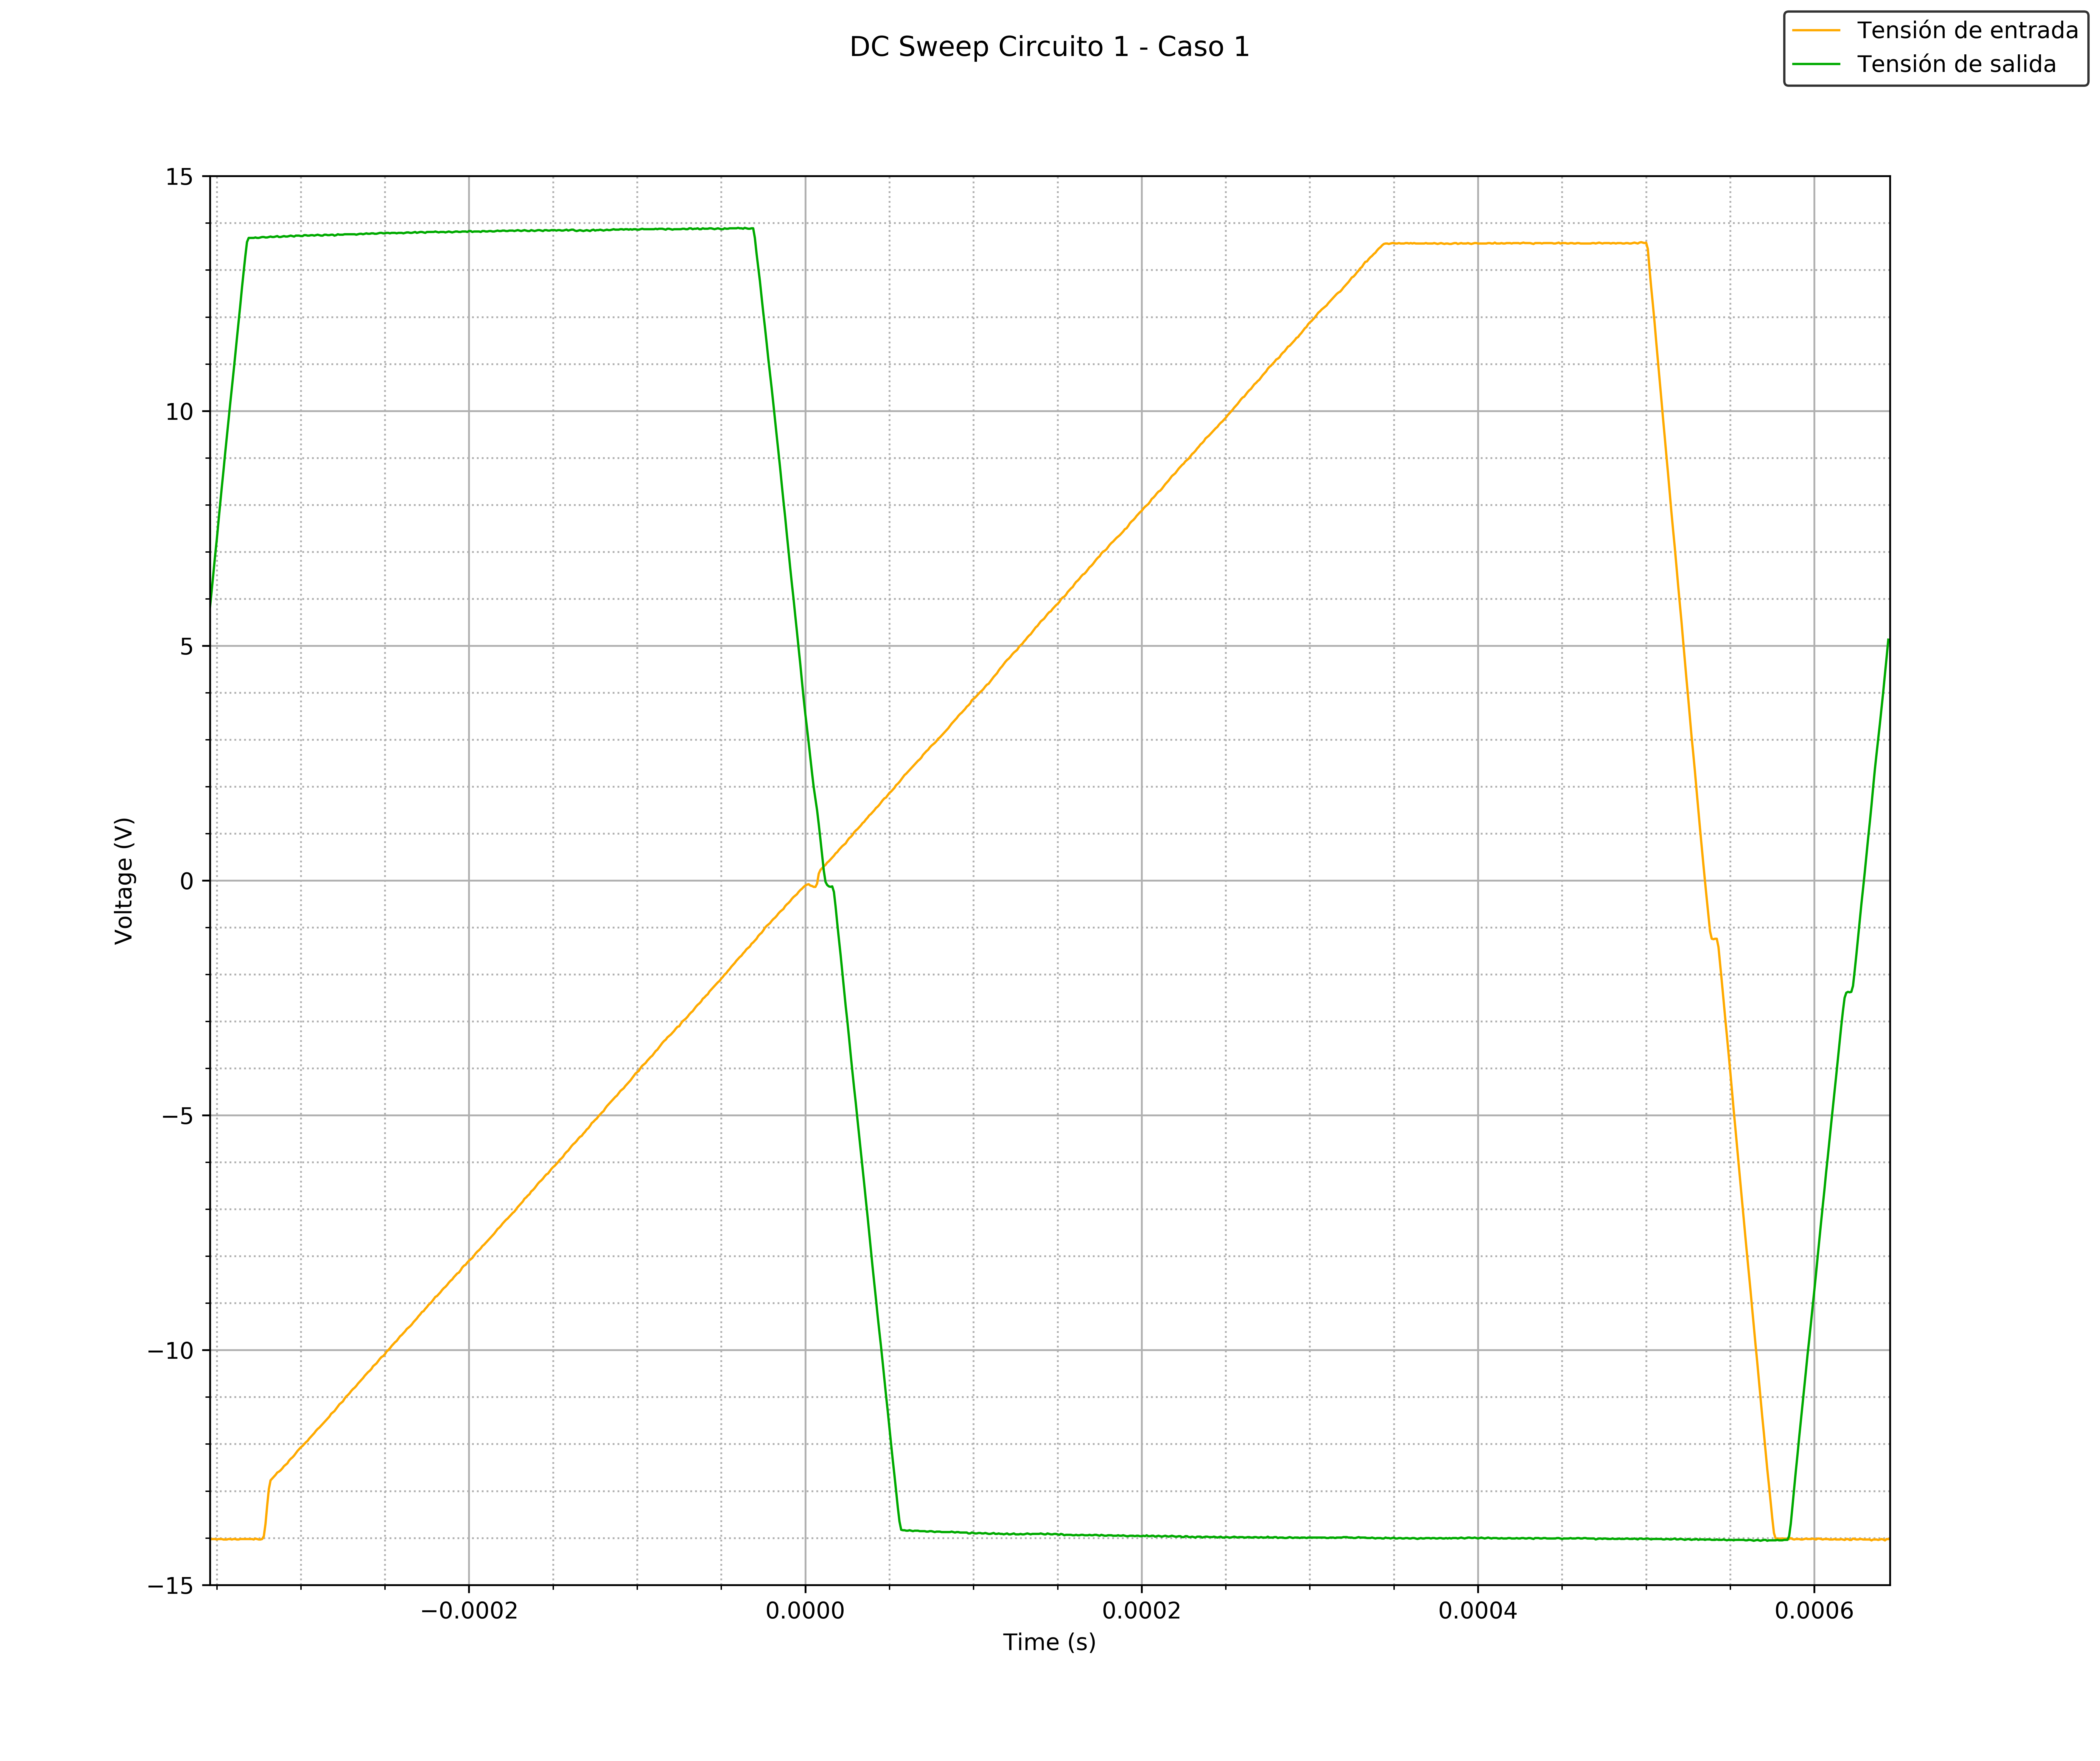
\includegraphics[width=10cm,height=10cm,keepaspectratio]{../EJ1/00GRAFICOS/c1dcs/c1c1dcs.png}
	\caption{DC Sweep del circuito inversor, caso 1.}
	\label{c1c1dcs}
\end{figure}

\begin{figure}[H] %!ht
	\centering
	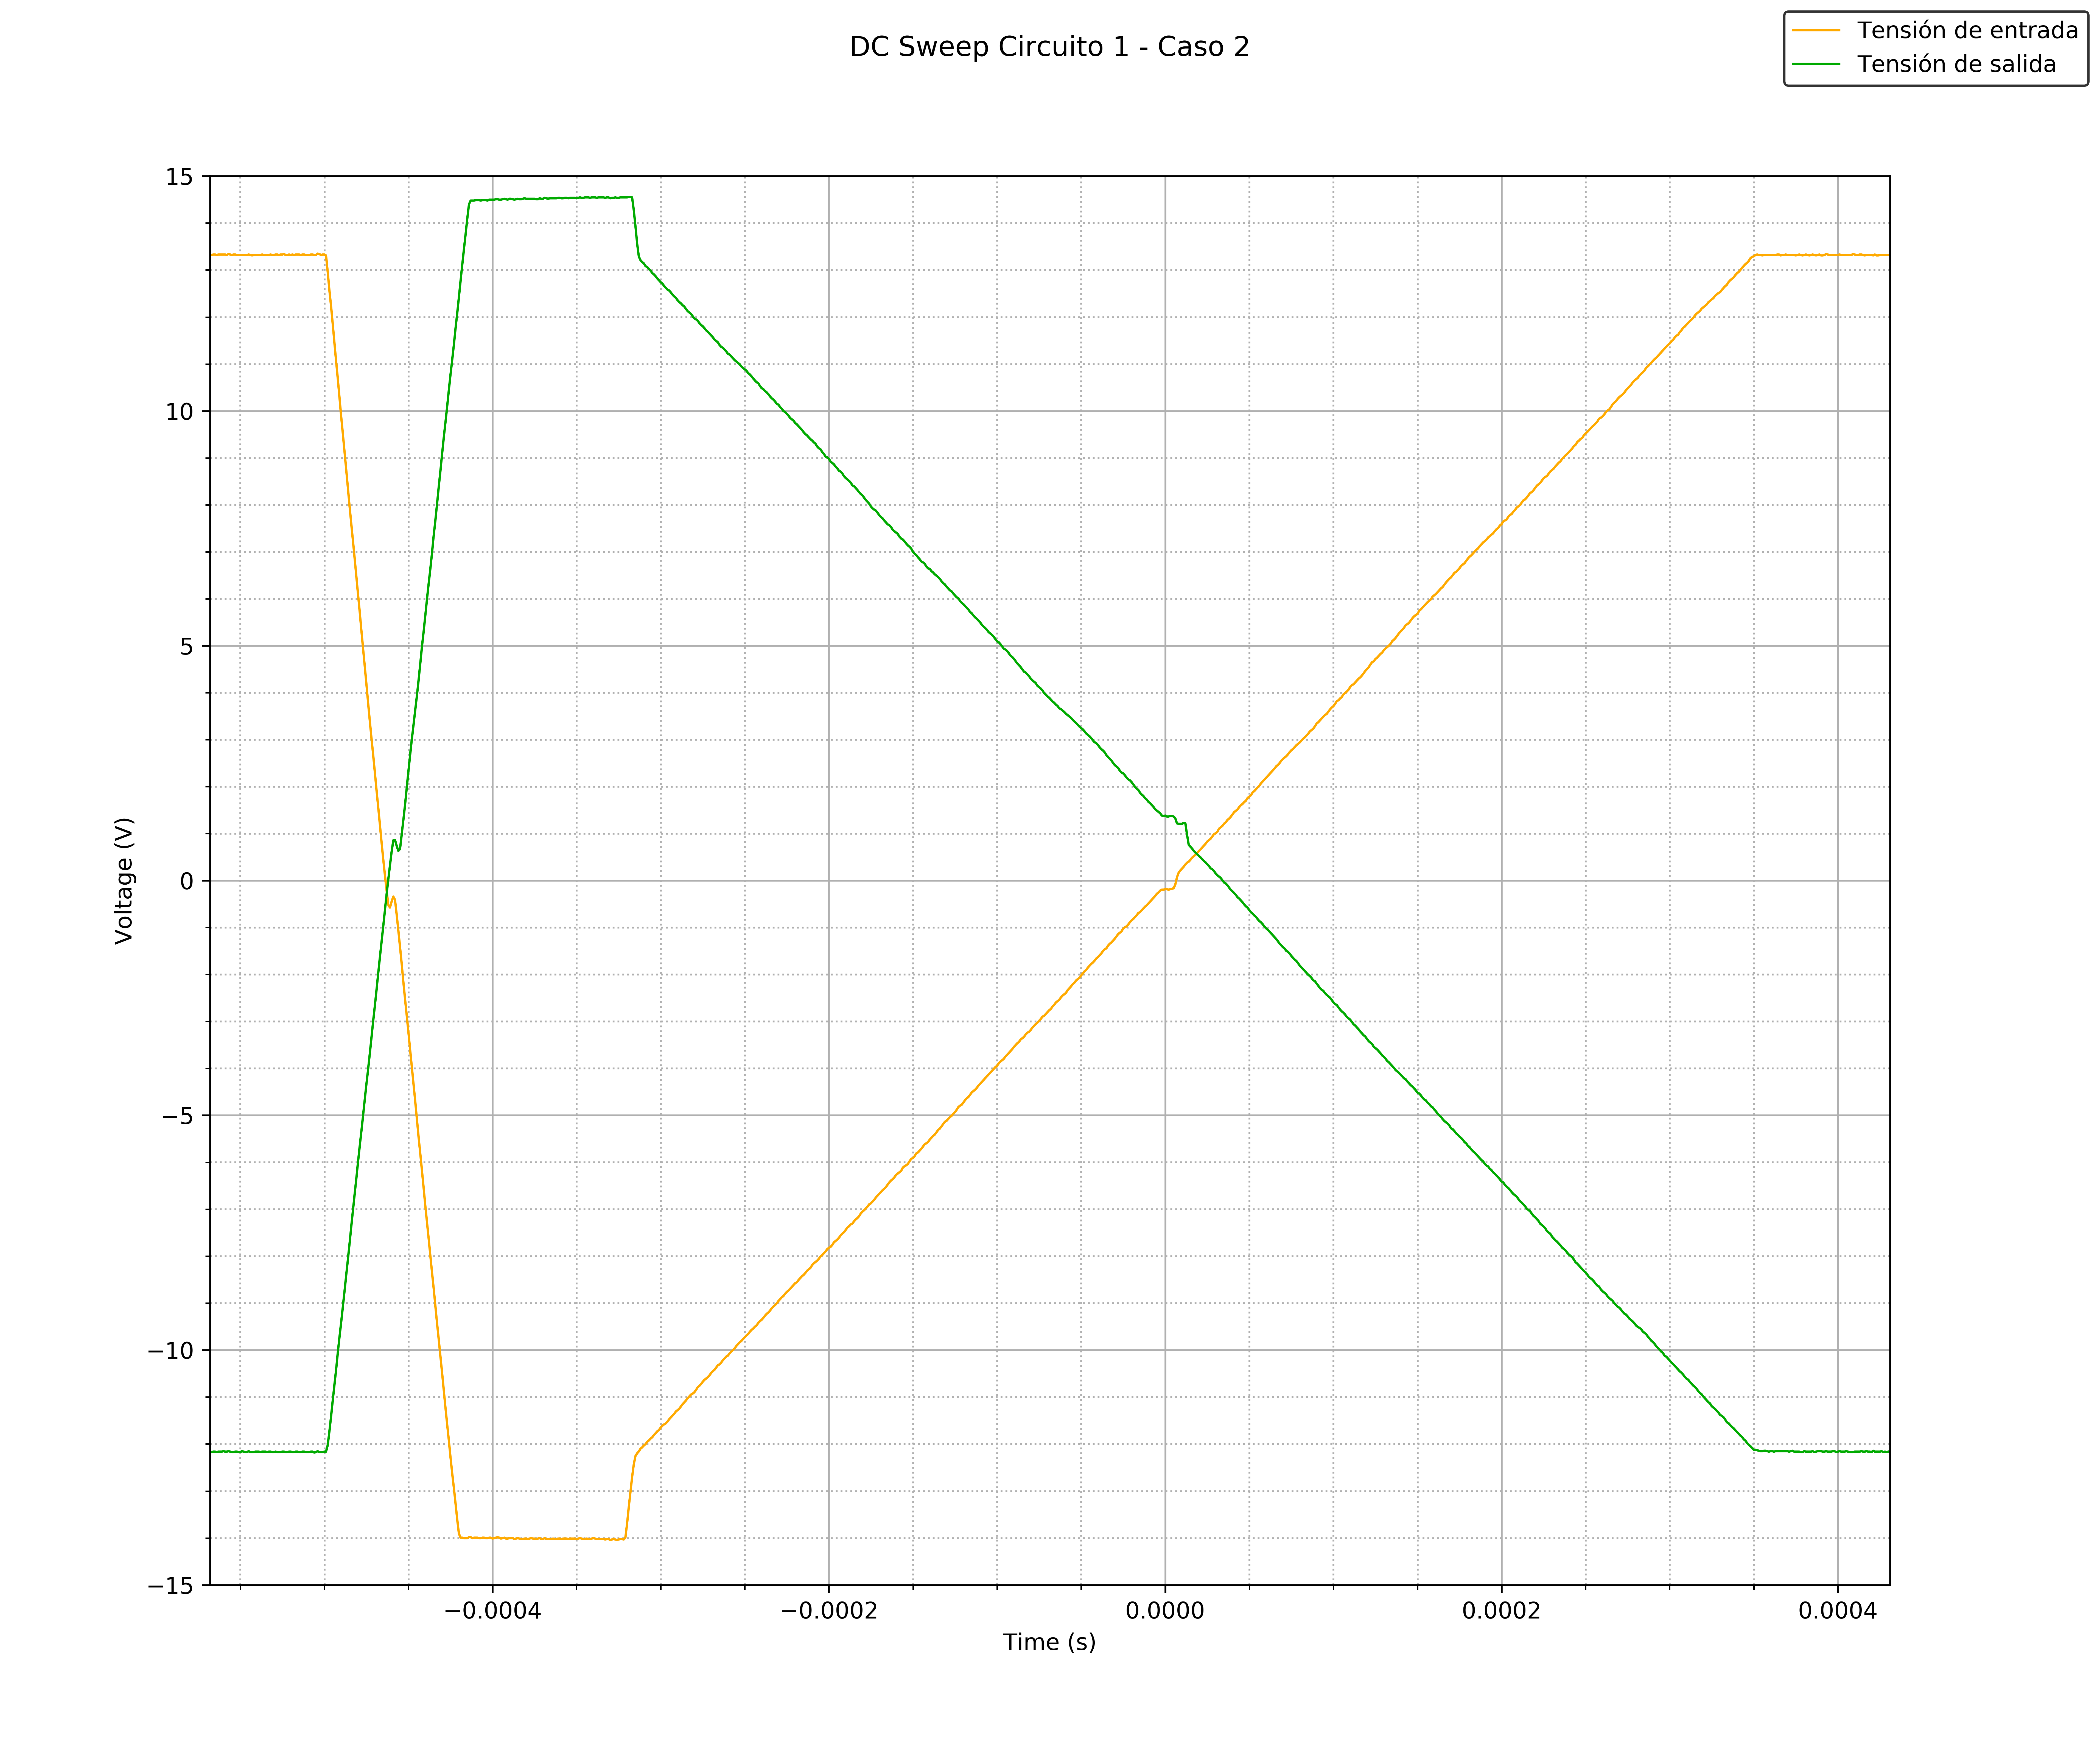
\includegraphics[width=10cm,height=10cm,keepaspectratio]{../EJ1/00GRAFICOS/c1dcs/c1c2dcs.png}
	\caption{DC Sweep del circuito inversor, caso 2.}
	\label{c1c2dcs}
\end{figure}

\begin{figure}[H] %!ht
	\centering
	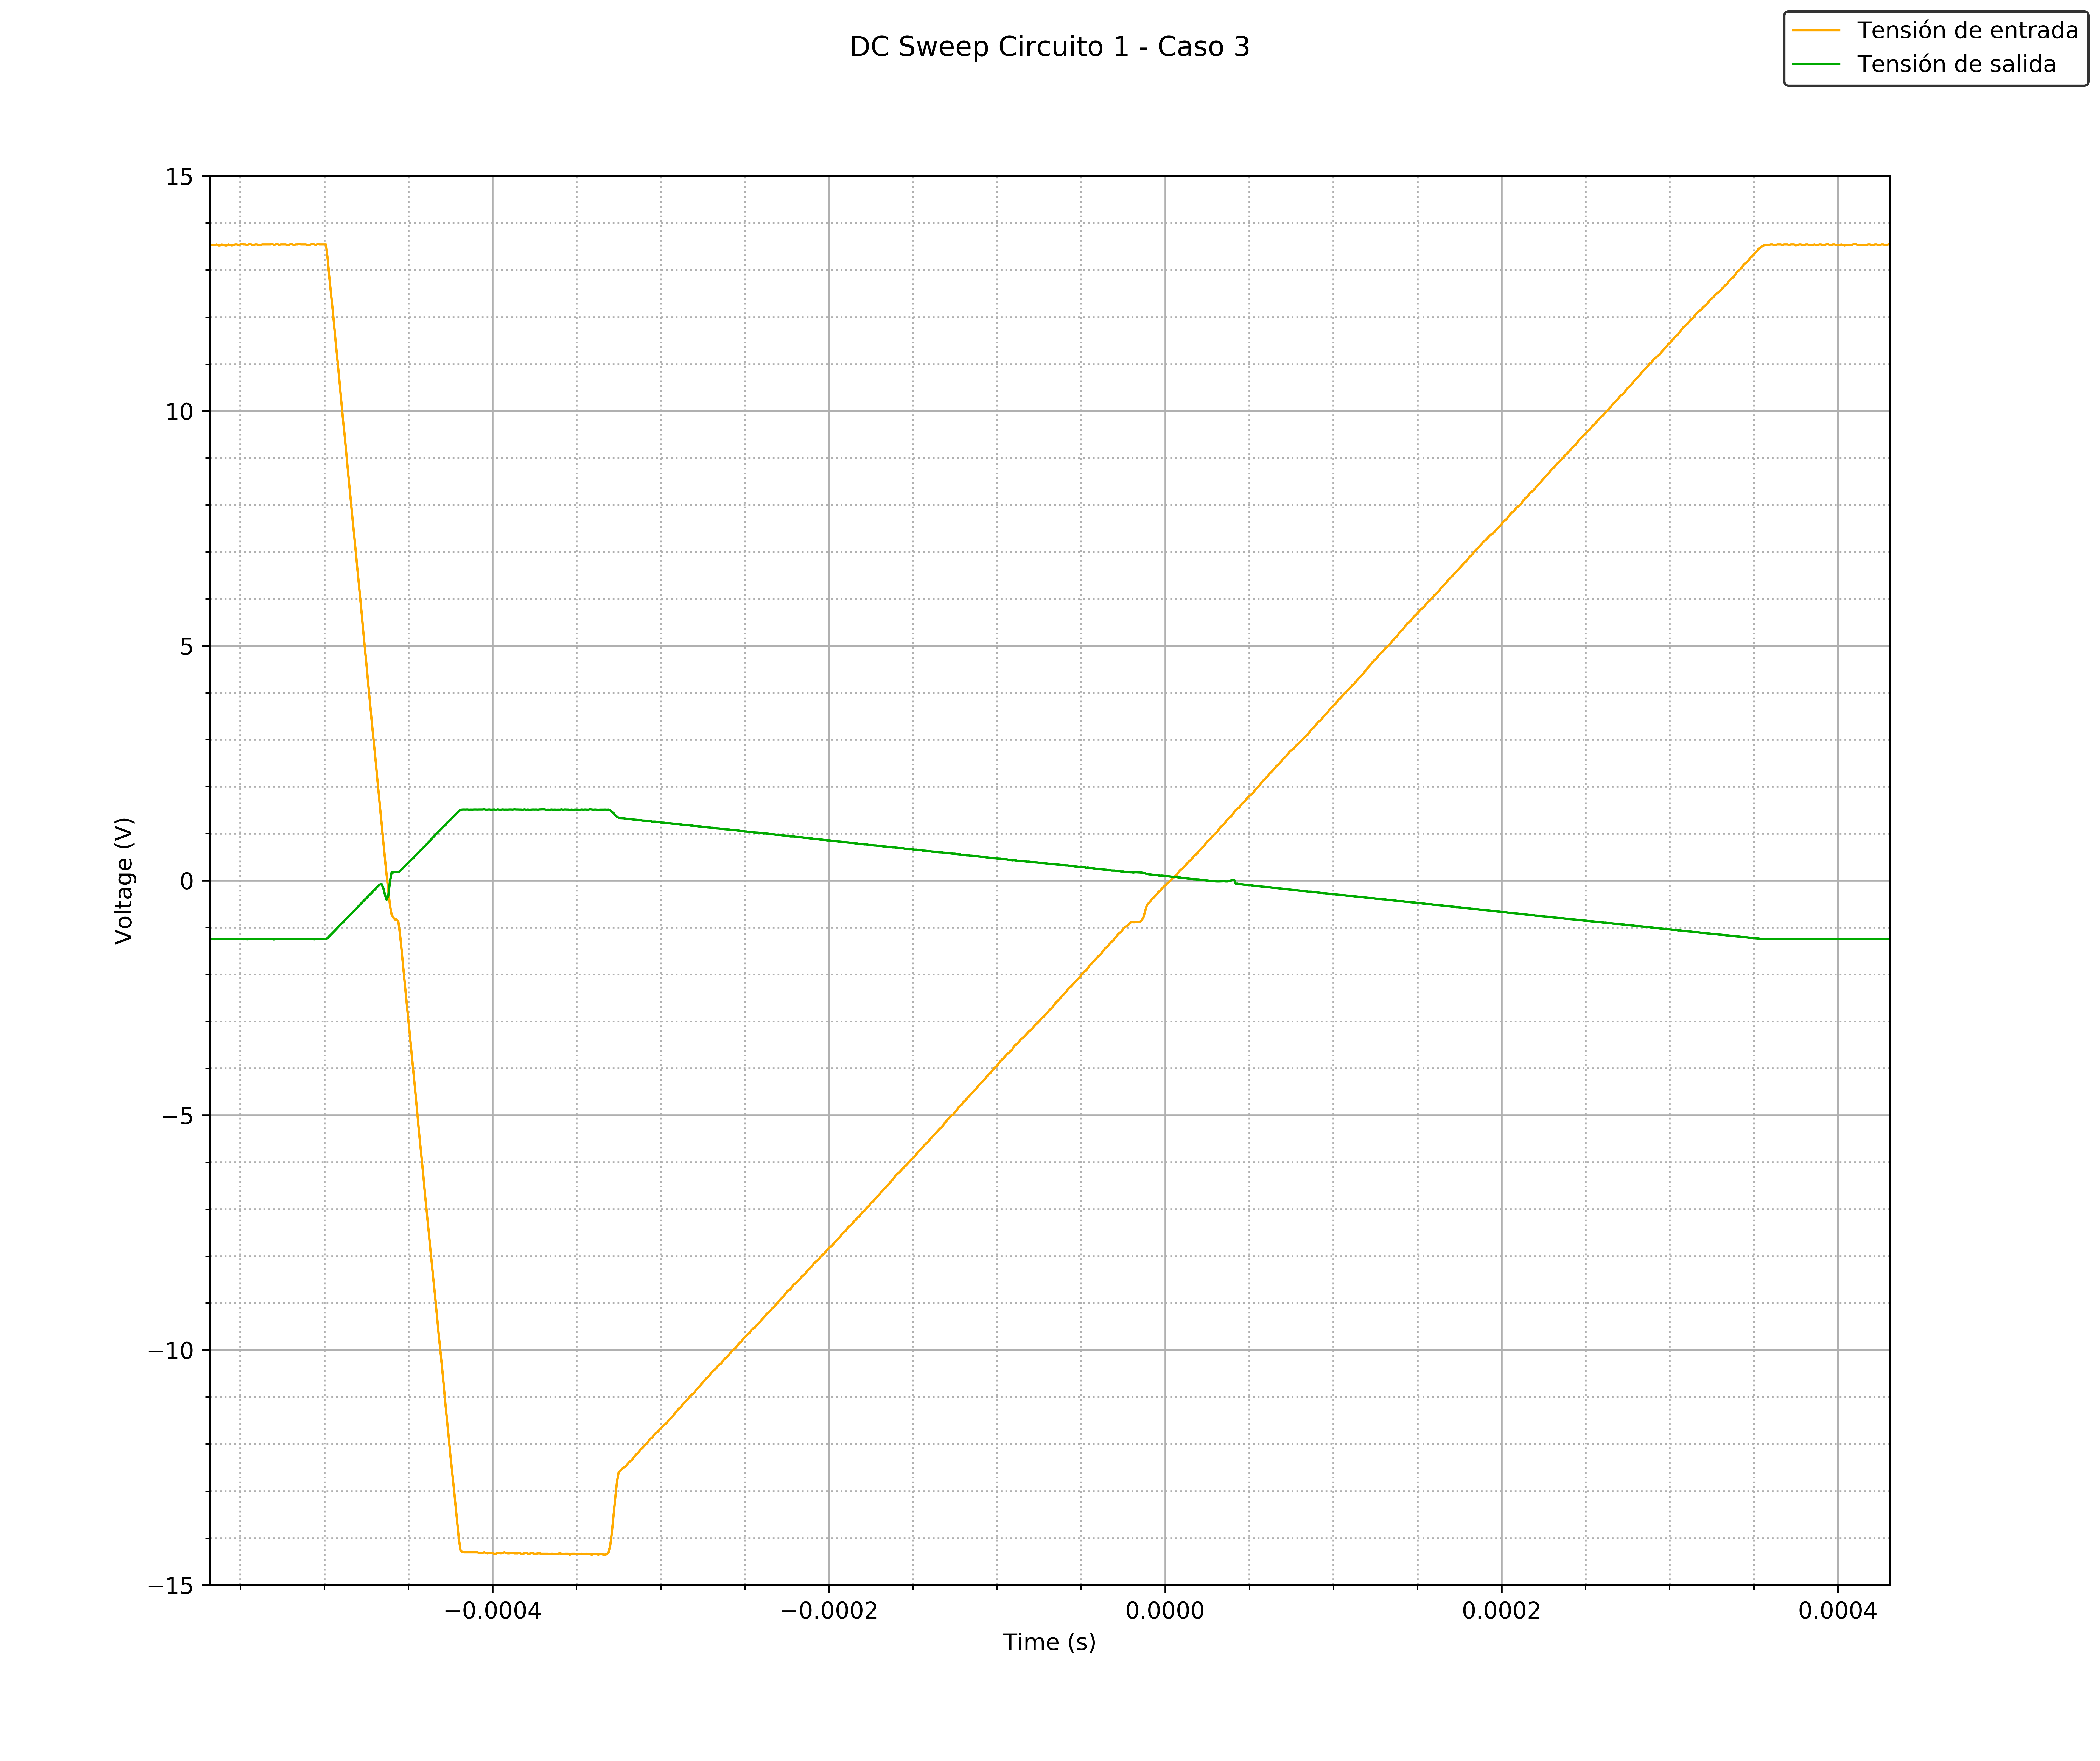
\includegraphics[width=10cm,height=10cm,keepaspectratio]{../EJ1/00GRAFICOS/c1dcs/c1c3dcs.png}
	\caption{DC Sweep del circuito inversor, caso 3.}
	\label{c1c2dcs}
\end{figure}

\subsubsection*{Configuraci\'on no inversora} %%%%%%%%%%%%%%%%%%%%%%%%%%

\begin{figure}[H] %!ht
	\centering
	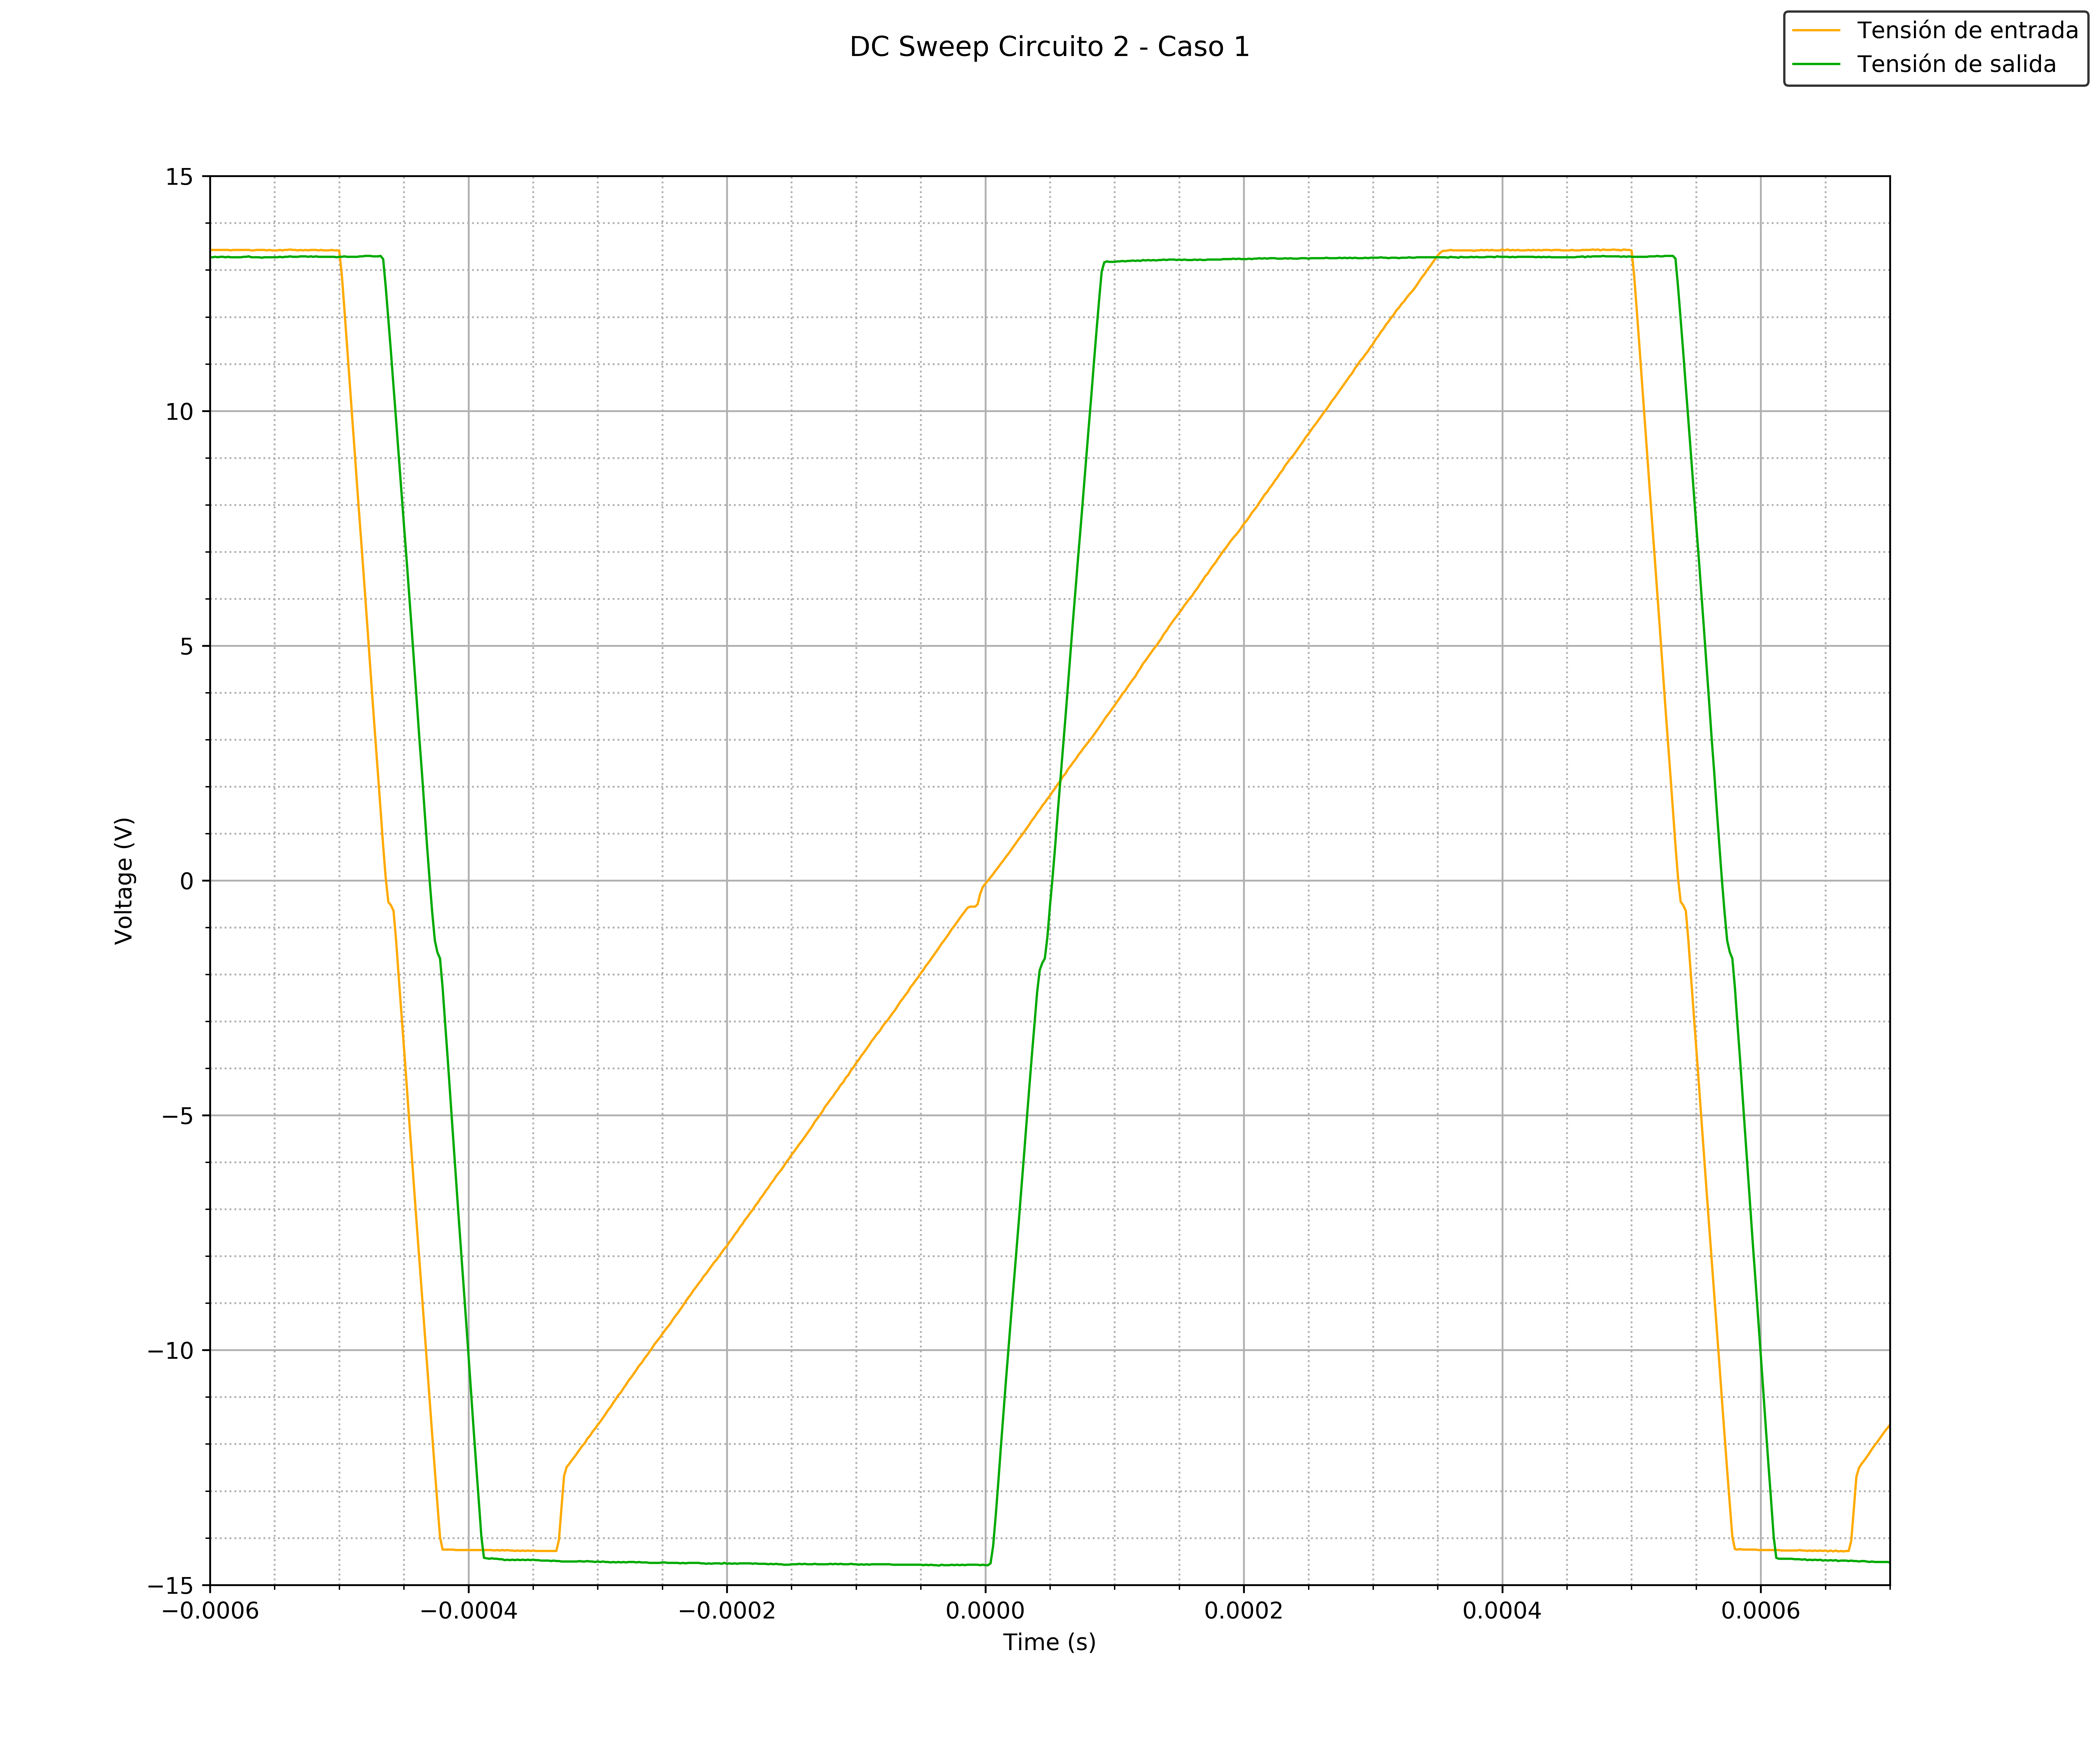
\includegraphics[width=10cm,height=10cm,keepaspectratio]{../EJ1/00GRAFICOS/c2dcs/c2c1dcs.png}
	\caption{DC Sweep del circuito no inversor, caso 1.}
	\label{c2c1dcs}
\end{figure}

\begin{figure}[H] %!ht
	\centering
	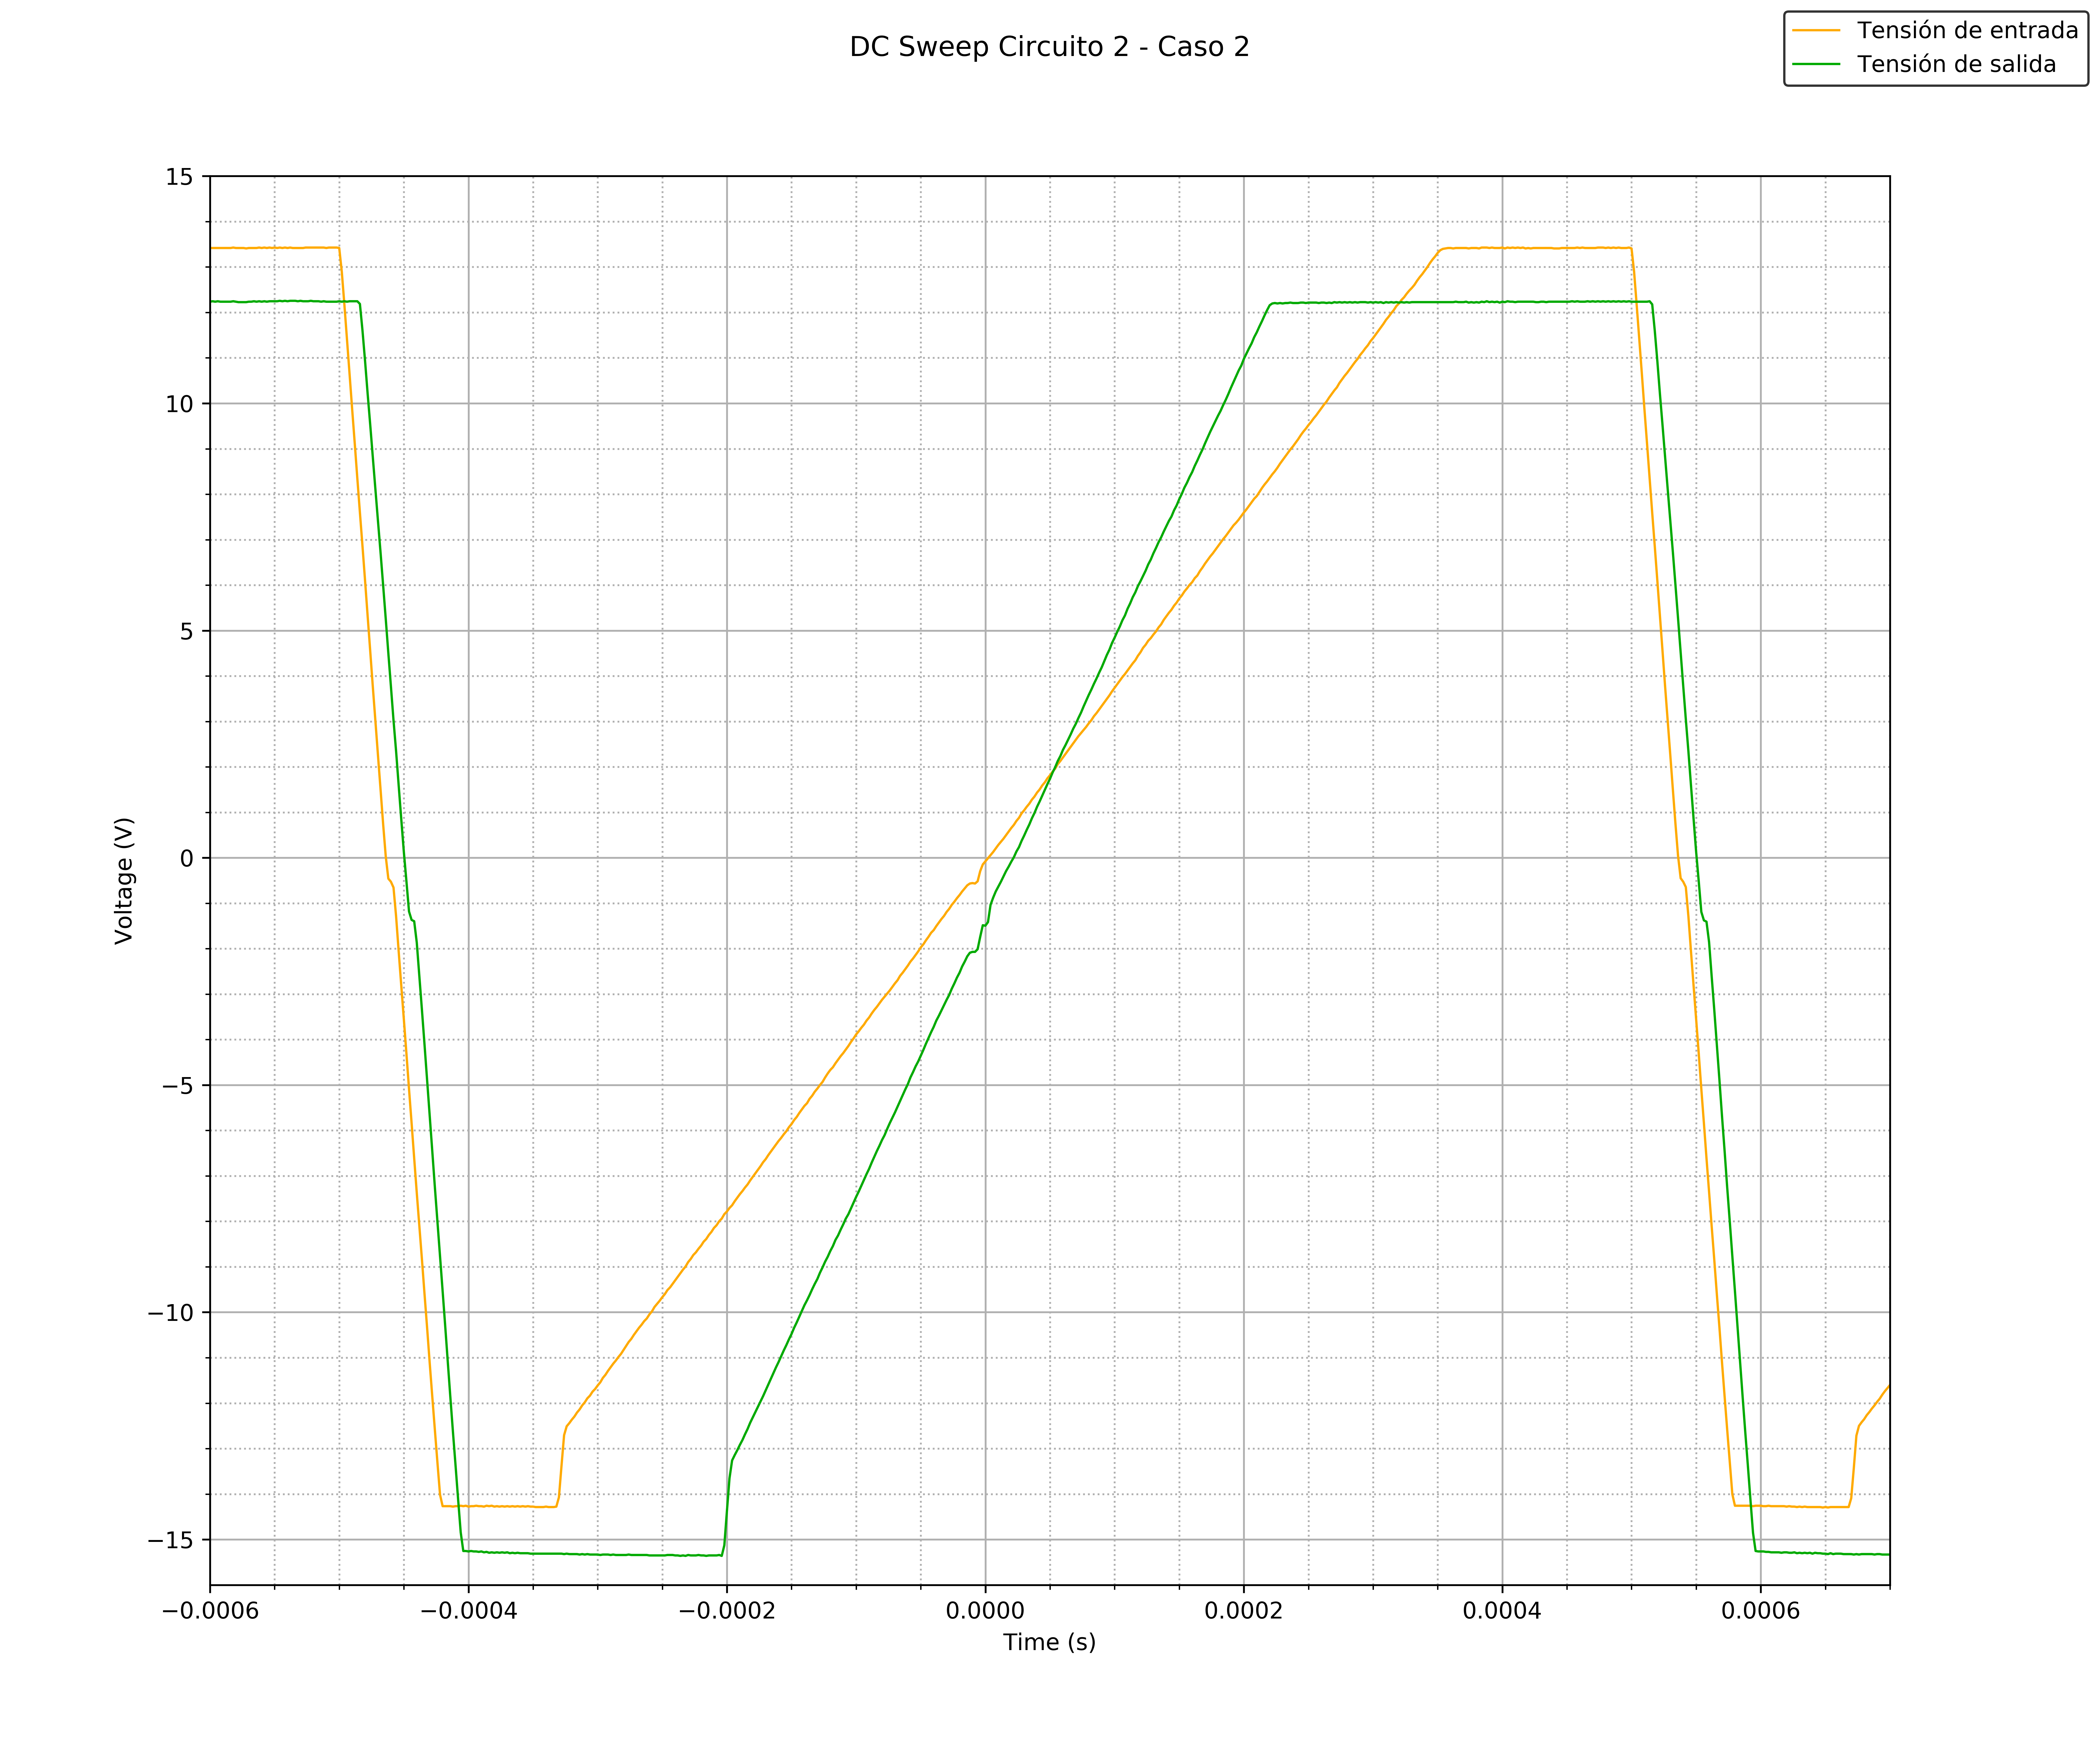
\includegraphics[width=10cm,height=10cm,keepaspectratio]{../EJ1/00GRAFICOS/c2dcs/c2c2dcs.png}
	\caption{DC Sweep del circuito no inversor, caso 2.}
	\label{c2c2dcs}
\end{figure}

\begin{figure}[H] %!ht
	\centering
	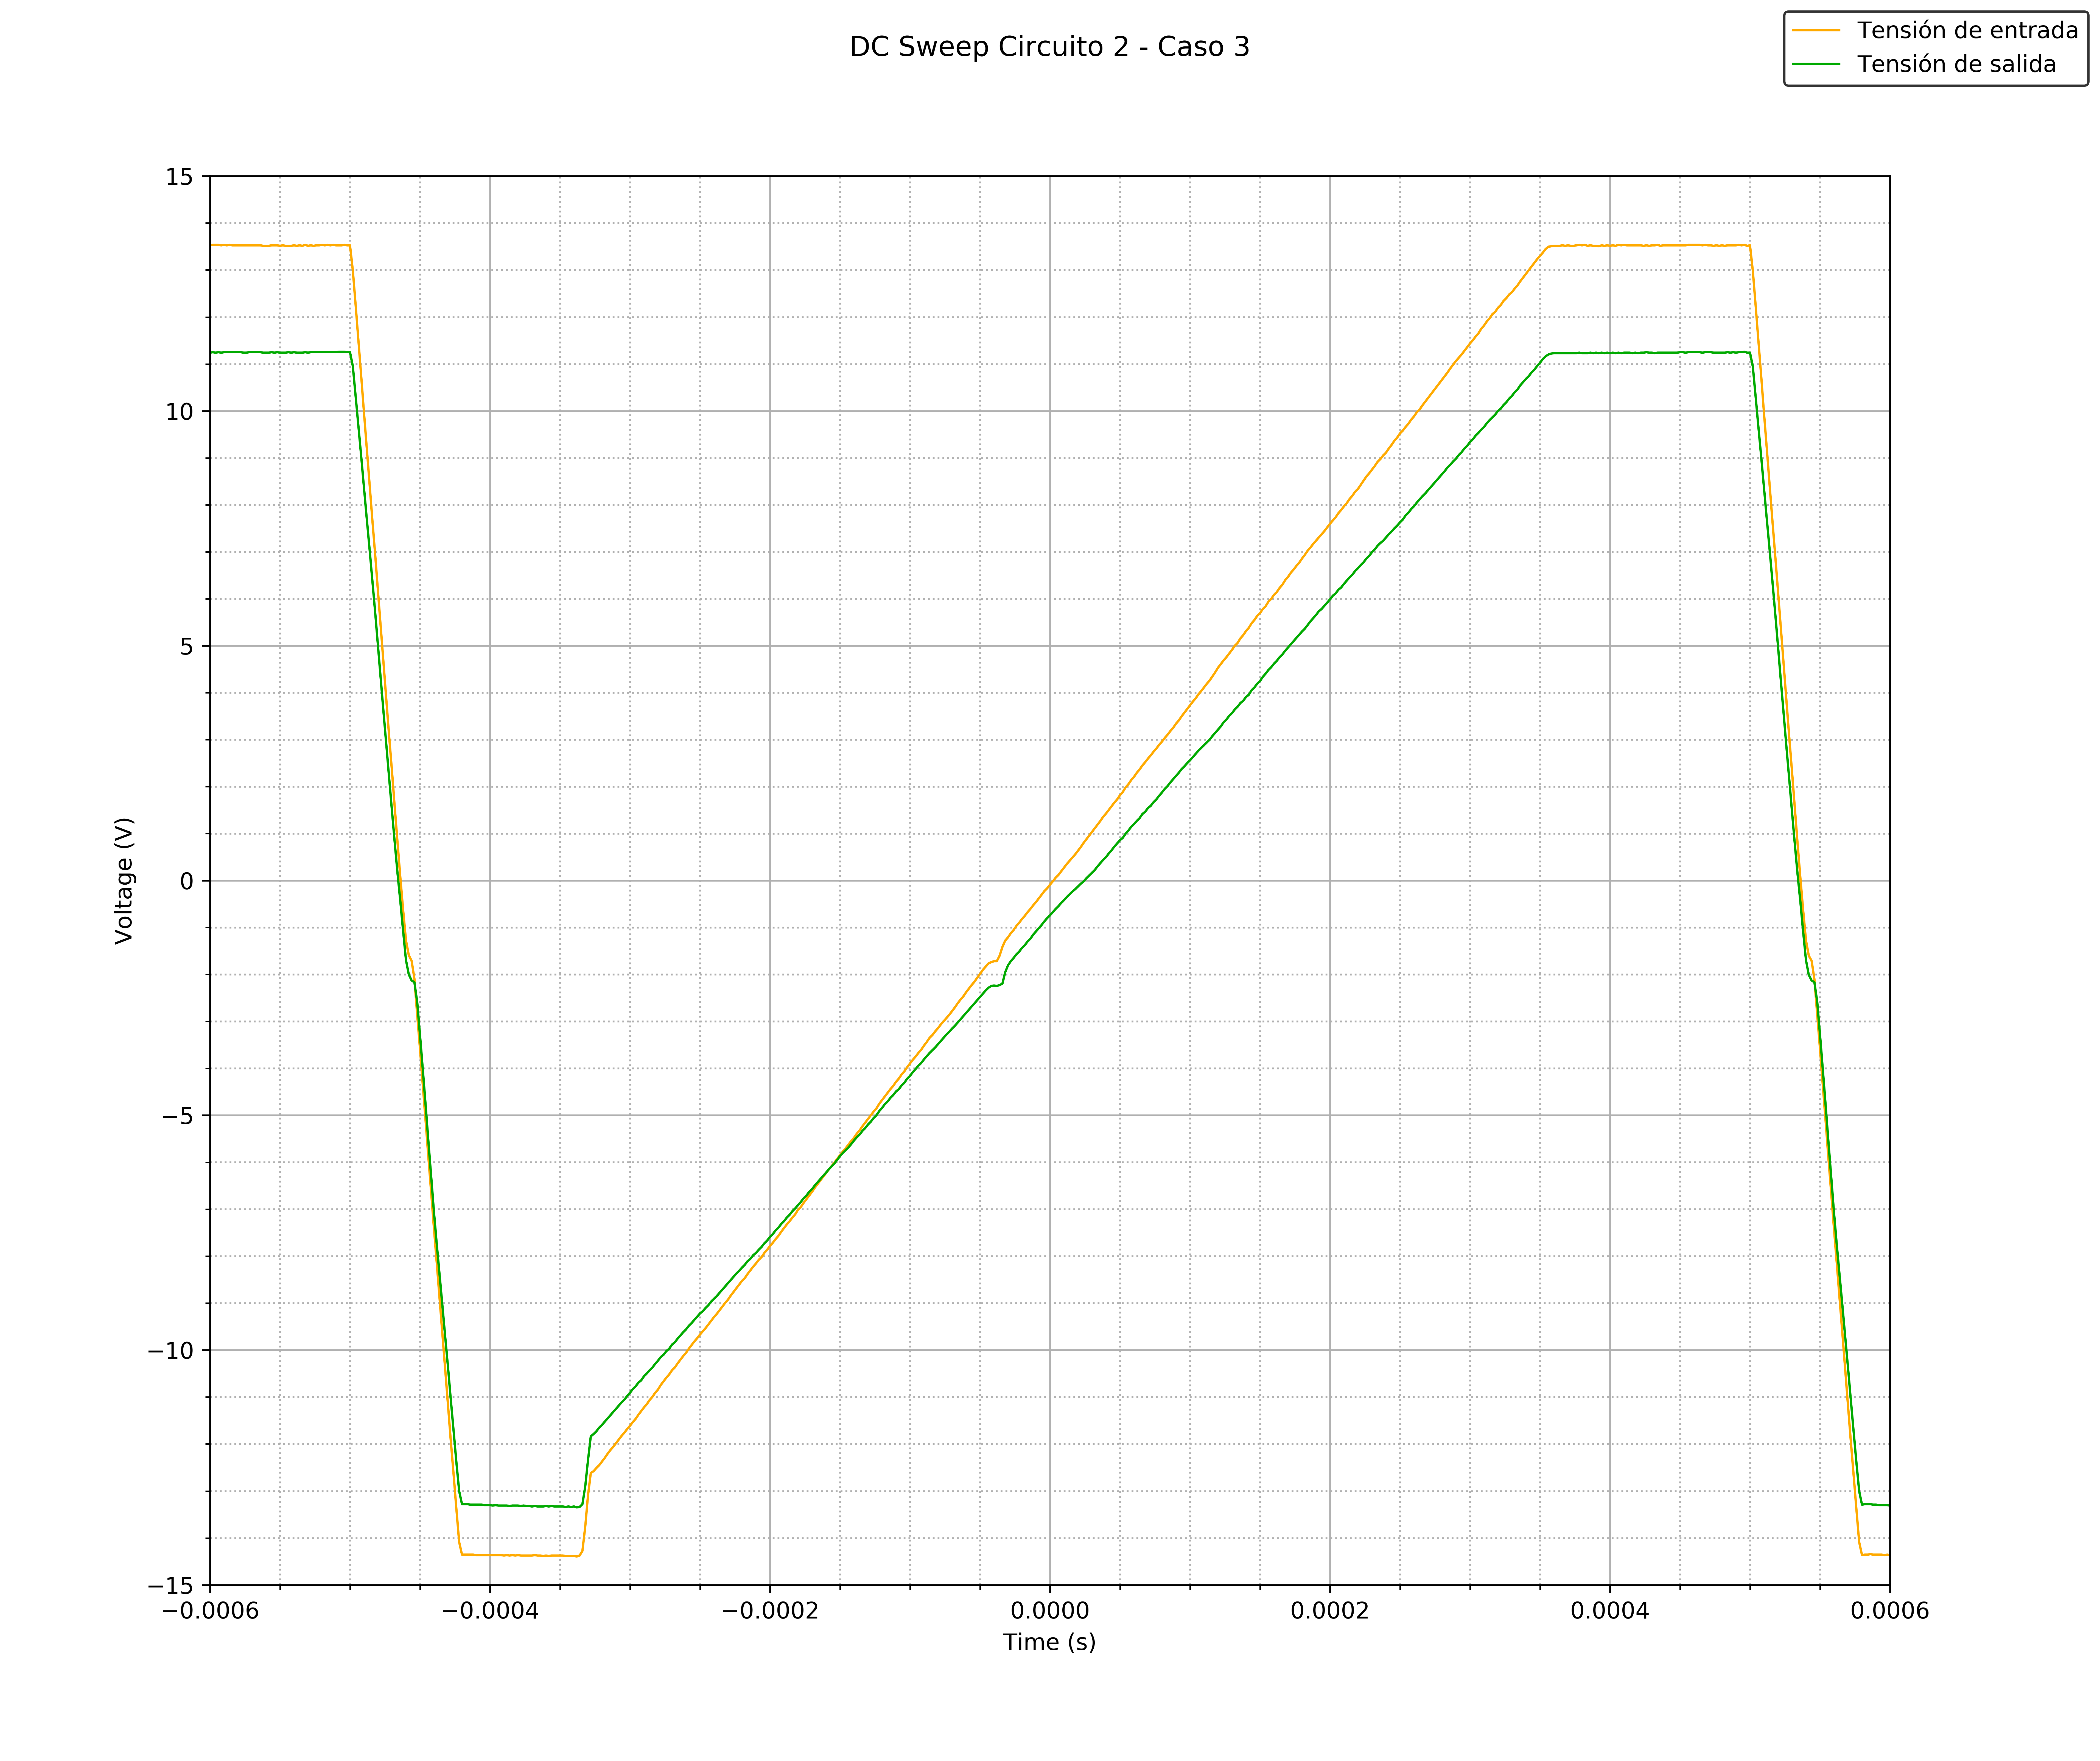
\includegraphics[width=10cm,height=10cm,keepaspectratio]{../EJ1/00GRAFICOS/c2dcs/c2c3dcs.png}
	\caption{DC Sweep del circuito no inversor, caso 3.}
	\label{c2c2dcs}
\end{figure}
%BUSCAR VALORES!!!!!!